%  !TeX  root  =  user_guide.tex

\section{MapServer Export Plugin}\label{sec:mapserver_export}

% when the revision of a section has been finalized,
% comment out the following line:
\updatedisclaimer

You can use QGIS to ``compose'' your map by adding and arranging layers,
symbolizing them, customizing the colors and then creating a map file
for MapServer.

\subsection{Creating the Project File}

The MapServer Export Plugin operates on a saved QGIS project file and
\textbf{not} on the current contents of the map canvas and legend. This
has been a source of confusion for a number of users. As described below,
before you start using the MapServer Export Plugin, you need to arrange
the raster and vector layers you want to use in MapServer and save this
status in a QGIS project file.

\begin{figure}[ht]
\centering
  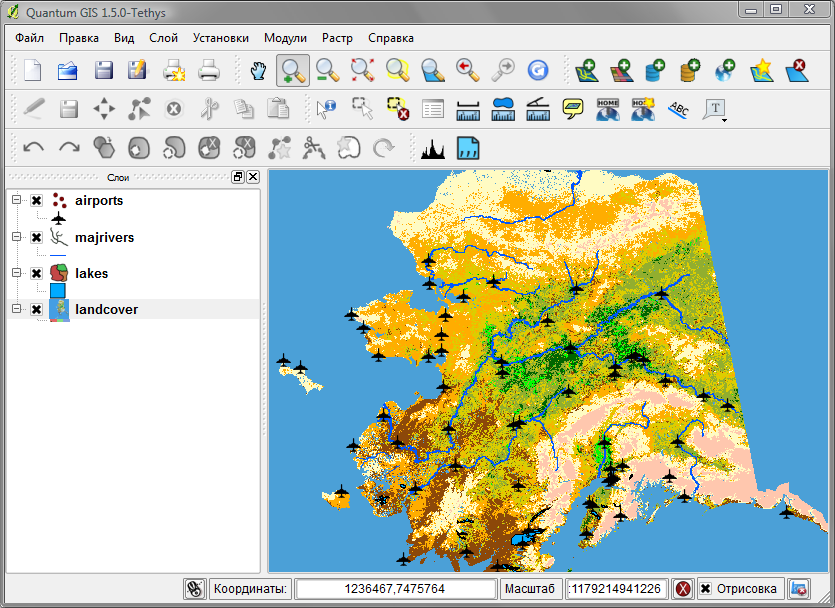
\includegraphics[clip=true, width=12cm]{mapserver_export_qgis}
   \caption{Arrange raster and vector layers for QGIS project file \nixcaption}
  \label{fig:mapserver_export_qgs}
\end{figure}

In this example, we demonstrate the four steps required to create a simple
project file which can be used to create the MapServer map file.
We use raster and vector files from the QGIS sample dataset \ref{label_sampledata}.

\begin{enumerate}
\item Add the raster layer \filename{landcover.tif} clicking on the
\toolbtntwo{mActionAddRasterLayer}{Add Raster Layer} icon.
\item Add the vector Shapefiles \filename{lakes.shp, majrivers.shp} and
\filename{airports.shp} from the QGIS sample dataset clicking on the
\toolbtntwo{mActionAddNonDbLayer}{Add Vector Layer} icon.
\item Change the colors and symbolize the data as you like (For example see
Figure~\ref{fig:mapserver_export_qgis})
\item Save a new project named \filename{mapserverproject.qgs} using
\mainmenuopt{File} \arrow \dropmenuopttwo{mActionFileSave}{Save Project}.
\end{enumerate}

\subsection{Creating the Map File}

The tool \filename{msexport} to export a QGIS project file to a MapServer map
file is installed in your QGIS binary directory and can be used independently of QGIS.
To use it from within QGIS, you need to enable the MapServer Export Plugin first using the Plugin Manager (see Section \ref{sec:load_core_plugin}).

\begin{figure}[ht]
\centering
  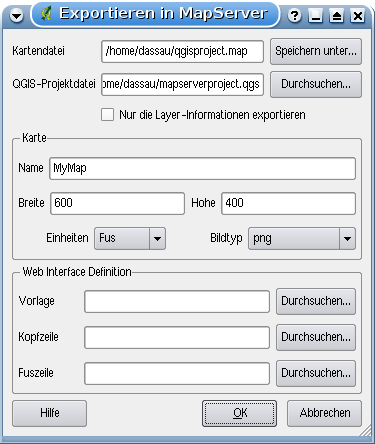
\includegraphics[clip=true, width=9cm]{mapserver_export_dialog}
  \caption{Export to MapServer Dialog \nixcaption}
  \label{fig:mapserver_export_dialog}
\end{figure}

\begin{description}
\item [Map file] \mbox{}\\
Enter the name for the map file to be created. You can use the button at the
right to browse for the directory where you want the map file created.
\item [Qgis project file] \mbox{}\\
Enter the full path to the QGIS project file (.qgs) you want to export. You can
use the button at the right to browse for the QGIS project file.
\item [Map Name] \mbox{}\\
A name for the map. This name is prefixed to all images generated by the mapserver.
\item [Map Width] \mbox{}\\
Width of the output image in pixels.
\item [Map Height] \mbox{}\\
Height of the output image in pixels.
\item [Map Units] \mbox{}\\
Units of measure used for output
\item [Image type] \mbox{}\\
Format for the output image generated by MapServer
\item [Web Template] \mbox{}\\
Full path to the MapServer template file to be used with the map file
\item [Web Header] \mbox{}\\
Full path to the MapServer header file to be used with the map file
\item [Web Footer] \mbox{}\\
Full path to the MapServer footer file to be used with the map file
\end{description}

Only the \filename{Map file} and \filename{QGIS project file} inputs are
required to create a map file, however by omitting the other parameters,
you may end up creating a non-functional map file, depending on your intended use.
Although QGIS is good at creating a map file from your project file,
it may require some tweaking to get the results you want.
For this example, we will create a map file using the project file
\filename{mapserverproject.qgs} we just created
(see Figure~\ref{fig:mapserver_export_dialog}):

\begin{enumerate}
  \item  Start the MapServer dialog (see
Figure \ref{fig:mapserver_export_dialog}) by clicking the \toolbtntwo{mapserver_export}{MapServer Export} icon in the toolbar menu.
  \item Enter the name (e.g., \filename{qgisproject.map}) for your new map file.
  \item Browse and find the QGIS project file (e.g., \filename{mapserverproject.qgs})
  you previously saved.
  \item Enter a name (e.g., \filename{MyMap}) for the map.
  \item Enter the width and height (e.g., \filename{600} for the width and \filename{400} for the height) for your output image.
  \item For this example, the layers are in meters, so we change the units to meters.
  \item Choose ``png'' for the image type.
  \item Click \button{OK} to generate the new map file \filename{qgisproject.map}.
  QGIS displays the success of your efforts.
\end{enumerate}

You can view the map file in any text editor or visualizer. If you
take a look, you'll notice that the export tool adds the metadata needed
to enable our map file for WMS.

\subsection{Testing the Map File}

We can now test our work using the \filename{shp2img} tool to create an image
from the map file. The \filename{shp2img} utility is part of MapServer and FWTools.
To create an image from our map:

\begin{itemize}[label=--]
\item Open a terminal window
\item If you didn't save your map file in your home directory, change to
  the folder where you saved it.
\item Run \filename{shp2img -m qgisproject.map -o mapserver\_test.png} and
  display the image
\end{itemize}

This creates a PNG with all the layers included in the QGIS project file.
In addition, the extent of the PNG will be the same as when we saved the
project. As you can see in Figure~\ref{fig:mapserver_export_test}, all
information except the airport symbols are included.

\begin{figure}[ht]
\centering
  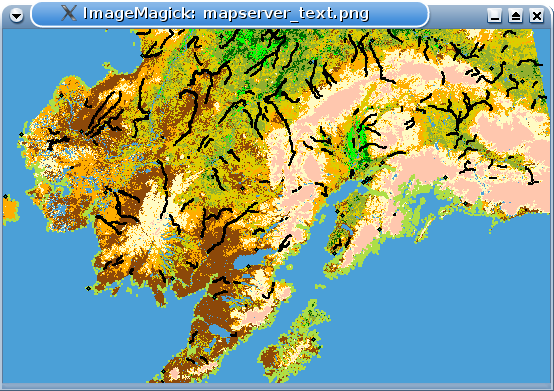
\includegraphics[clip=true, width=10cm]{mapserver_export_test}
  \caption{Test PNG created by shp2img with all MapServer Export layers \nixcaption}
  \label{fig:mapserver_export_test}
\end{figure}

If you plan to use the map file to serve WMS requests, you probably don't
have to tweak anything. If you plan to use it with a mapping template or a
custom interface, you may have a bit of manual work to do. To see how easy
it is to go from QGIS to serving maps on the web, take a look at
Christopher Schmidt's 5 minute flash video. He used an older version of QGIS (version 0.8), but the demo applies equally well to newer versions.
\footnote{\url{http://openlayers.org/presentations/mappingyourdata/}}

\FloatBarrier
